\documentclass[	%----------------------Preamble---------------------------------------------------%
		11pt,a4paper,	% fontsize and papersize
		twoside,		% double sided layout
		english,		% document language (also numberingsystem)
		f1				% HsH facultie
	]{HsH-report}		% documentclass

\usepackage{color}		% for coloring stuff
\usepackage{siunitx}	% units
\usepackage{biblatex}	% bibiography
\addbibresource{src/localBibliography.bib}

\usepackage{lipsum}		% dummy text
\begin{document}

\pagenumbering{Roman}	% duífferent numbering until first chapter
\maketitle				% using personal.tex
\declarationAuthorship

\begin{abstract}
	\lipsum[5-8]
\end{abstract}

\tableofcontents

\cleardoublepage % importand when using double sided layout
\pagenumbering{arabic} % numbering in normal numbers

\chapter{Examples}
	\label{chap: one}
	{\color{red}red text} and {\color{blue}blue text} \\
	different subscripts: \normalsubscripts$R_t$ \upsubscripts$R_t$ \\
	using Units: $R=200\,\milli\ohm + \SI{0.34567453}{\volt\per\metre} - 5\,\si{\second\per\metre\squared}$ \\
	some information\cite{laboranleitung:physik}\\
	german number: $3,5$ english number: $3.5$\\
	\begin{figure}
		\centering
		
\includegraphics[width=.6\textwidth]{img/lorem-ipsum.jpg}
		\caption{test}
	\end{figure}

	\begin{figure}
		\centering
		\includegraphics[width=0.6\textwidth, page=2]{plt/build/examplePlot.pdf}
		\caption{a nice plot}
	\end{figure}

	\begin{figure}
		\centering
		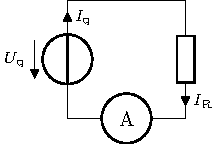
\includegraphics{crc/build/exampleCircuit.pdf}
		\caption{a circuit diagramm}
	\end{figure}

	\begin{figure}
		\centering
		\graphicspath{{svg/build/}} % double curly brackets needet for unknown reason
		\input{svg/build/exampleSVG.pdf_tex}
		\caption{made via inkscape}
	\end{figure}

\chapter{Using formulas}
	\label{chap: theorie}
	a numberd formula:
	\begin{equation}
		\label{eq: einhalb} % always lable your stuff
		0,5=\frac{1}{3}
	\end{equation}
	\autoref{eq: einhalb} is nice, but how about multiple lines:
	\begin{equation}
	\begin{split} % you need do nest this
		x &= x^2+3 \\
		\Leftrightarrow 0 &= x^2-x+3 \\
	\end{split}
	\end{equation}
	and jow could you align formulas?
	\begin{align}
		x_1 &= 6 &&|\;\mbox{mit } x \in \mathbb{N} \\
		x_2 &= 33+\abs{\frac{1}{4}} &&|\;x_1+3 \\
			&= 33,25 &&\mbox{| warum alles numerieren?} \notag \\
		x_3 &= 10^{22}
	\end{align}


\printbibliography
\listoffigures
\end{document}
